\chapter{Fotoquímica}\label{ch:b3:photochemistry}

A visão começa quando um fóton dobra uma molécula. Nos bastonetes do olho, o
retinal está alojado em sua proteína na forma 11-cis; um fóton de luz verde o
transforma na forma todo-trans, e a isomerização se completa essencialmente em
\qty{200}{fs}, mais depressa que quase qualquer outro evento químico. O resto da
visão, uma enorme amplificação bioquímica, decorre dessa única molécula dobrada.
As mesmas regras (um fóton excita uma molécula, que então escolhe entre vários
destinos) governam os protetores solares, a síntese de anéis tensionados, a
terapia fotodinâmica, o smog sobre as cidades e a \omterm{def:b3:photochemistry:chapman}{camada de ozônio} que protege
a superfície da Terra da luz ultravioleta.

\begin{recall}
O \cref{ch:b3:electronic-spectroscopy} descreveu os estados excitados das
moléculas, o \omterm{def:b3:electronic-spectroscopy:jablonski}{diagrama de Jablonski}, o \omterm{def:b3:electronic-spectroscopy:radiationless}{cruzamento intersistemas}, a \omterm{def:b3:electronic-spectroscopy:luminescence}{fluorescência}
e a \omterm{def:b3:electronic-spectroscopy:luminescence}{fosforescência}, a supressão e o \omterm{def:b3:electronic-spectroscopy:quantum-yield}{rendimento quântico} de um processo
fotofísico. O volume do 1.º ano definiu os radicais, a homólise e os isômeros
$Z$/$E$; o volume do 2.º ano, as reações concertadas, os orbitais de fronteira e
os ciclos catalíticos. O \cref{ch:b3:complex-kinetics} tratou das \omterm{def:b3:complex-kinetics:chain}{reações em
cadeia} e dos estados estacionários.
\end{recall}

\section{A luz como reagente}

Dois princípios antigos abrem o assunto: só a luz absorvida pode causar uma
transformação química (Grotthuss e Draper), e cada fóton absorvido excita uma
molécula (Stark e Einstein).

\begin{definition}[Fluxo de fótons, actinômetro químico]\label{def:b3:photochemistry:photon-flux}
O \emph{fluxo de fótons}\index{fluxo de fotons@fluxo de fótons} de uma fonte de luz é o número de
fótons que ela fornece por unidade de tempo, muitas vezes contado em mols de
fótons (einstein) por segundo. Um \emph{actinômetro químico}\index{actinometro quimico@actinômetro químico} é
uma reação fotoquímica de \omterm{def:b3:electronic-spectroscopy:quantum-yield}{rendimento quântico} conhecido com precisão, usada para
medir um fluxo de fótons.
\end{definition}

\begin{proposition}[Lei de Stark--Einstein]\label{prop:b3:photochemistry:stark-einstein}
Nas intensidades de luz usuais, cada fóton absorvido excita exatamente uma
molécula; os \omterm{def:b3:electronic-spectroscopy:quantum-yield}{rendimentos quânticos} primários de todos os processos que partem do
estado excitado somam 1.
\end{proposition}

\begin{proof}[Demonstração parcial]
Que um fóton seja absorvido por uma molécula de cada vez é admitido (a absorção
de dois fótons exige as intensidades dos lasers pulsados). A molécula excitada
desaparece então por processos de primeira ordem concorrentes, de constantes de
velocidade $k_i$ (\cref{ch:b3:electronic-spectroscopy}): a fração que segue o
caminho $i$ é $\Phi_i =
k_i/\sum_jk_j$, e $\sum_i\Phi_i = 1$.
\end{proof}

O \omterm{def:b3:electronic-spectroscopy:quantum-yield}{rendimento quântico} de uma reação, o número de moléculas convertidas por fóton
absorvido, não precisa obedecer a esse limite: uma etapa fotoquímica primária
pode iniciar uma cadeia. Uma mistura de \ce{H2} e \ce{Cl2} exposta à luz reage com
\omterm{def:b3:electronic-spectroscopy:quantum-yield}{rendimentos quânticos} de $10^4$ e mais, cada \ce{Cl2} fotolisado iniciando uma
cadeia como a da reação hidrogênio--bromo do \cref{ch:b3:complex-kinetics}; um
\omterm{def:b3:electronic-spectroscopy:quantum-yield}{rendimento quântico} maior que 1 é a assinatura de uma cadeia.

\begin{proposition}[Velocidade de uma reação fotoquímica]\label{prop:b3:photochemistry:rate}
Uma solução de absorbância $A$ no comprimento de onda de irradiação, que recebe um
\omterm{def:b3:photochemistry:photon-flux}{fluxo de fótons} $I_0$ (einstein por segundo), absorve $I_{\mathrm{abs}} = I_0(1 - 10^{-A})$; se o
reagente absorve tudo, a reação converte $v = \Phi I_{\mathrm{abs}}$ mols por segundo.
\end{proposition}

\begin{proof}
Pela lei de Beer--Lambert, o fluxo transmitido é $I_010^{-A}$, logo o absorvido é
$I_0(1 - 10^{-A})$; pela definição do \omterm{def:b3:electronic-spectroscopy:quantum-yield}{rendimento quântico}, $\Phi$ moléculas reagem por
fóton absorvido.
\end{proof}

\begin{method}[A velocidade de uma fotorreação a partir da lâmpada]\label{met:b3:photochemistry:photochemical-rate}
\begin{enumerate}
  \item Energia do fóton $E = hc/\lambda$; \omterm{def:b3:photochemistry:photon-flux}{fluxo de fótons} $I_0 = P/E$ para uma potência $P$ que
        chega à amostra, ou medido com um actinômetro; divida por $N_A$ para obter
        einstein por segundo.
  \item Fração absorvida $1 - 10^{-A}$, com $A$ no comprimento de onda de irradiação (ela
        muda à medida que o reagente é consumido).
  \item Velocidade $\Phi I_{\mathrm{abs}}$ em mol/s, dividida pelo volume para uma velocidade em concentração.
\end{enumerate}
\end{method}

\begin{method}[Actinometria com ferrioxalato]\label{met:b3:photochemistry:actinometry}
\begin{enumerate}
  \item Irradie, na mesma cubeta e com a mesma geometria do experimento, uma solução
        acidificada de tris(oxalato)ferrato(III) de potássio, concentrada o bastante
        para absorver praticamente toda a luz abaixo de cerca de \qty{450}{nm}.
  \item A luz reduz Fe(III) a Fe(II) com um \omterm{def:b3:electronic-spectroscopy:quantum-yield}{rendimento quântico} calibrado; depois
        de um tempo medido, adicione 1,10-fenantrolina e tampão, e meça a
        absorbância do complexo vermelho $\ce{[Fe(phen)3]^{2+}}$.
  \item Os mols de Fe(II) divididos por (\omterm{def:b3:electronic-spectroscopy:quantum-yield}{rendimento quântico} $\times$ tempo) dão o \omterm{def:b3:photochemistry:photon-flux}{fluxo de fótons}.
\end{enumerate}
\end{method}

\section{Reações fotoquímicas}

\begin{definition}[Fotoisomerização, estado fotoestacionário]\label{def:b3:photochemistry:photoisomerisation}
Uma \emph{fotoisomerização}\index{fotoisomerizacao@fotoisomerização} é uma conversão
induzida pela luz de um isômero em outro, tipicamente $E \to Z$ em torno de uma
ligação dupla. Sob irradiação contínua, dois isômeros que absorvem ambos atingem um
\emph{estado fotoestacionário}\index{estado fotoestacionario@estado fotoestacionário}, uma composição estável
fixada pela luz, e não pela termodinâmica.
\end{definition}

A torção de uma ligação dupla explica por que a luz isomeriza os alcenos. No
estado fundamental, a energia sobe à medida que as duas extremidades se torcem,
até um máximo em $90^\circ$, onde a ligação $\pi$ está rompida. No estado excitado
$\pi\pi^*$, a ordem se inverte: a geometria torcida é a mais estável. Uma molécula
excitada se torce em direção a $90^\circ$, onde as duas superfícies se aproximam,
volta ali ao estado fundamental e cai para um dos lados: para o isômero de
partida ou para o outro.

\begin{omfigure}
\begin{tikzpicture}[font=\small, >=Stealth, x=0.032cm, y=1.1cm]
  \draw[->] (0,0) -- (195,0);
  \node[anchor=north] at (135,-0.45) {ângulo de torção};
  \draw[->] (0,0) -- (0,5.2) node[anchor=south] {energia};
  \foreach \t/\l in {0/{0^\circ}, 90/{90^\circ}, 180/{180^\circ}}{
    \draw (\t,0) -- (\t,-0.08) node[anchor=north] {$\l$};}
  \draw[thick, black, domain=0:180, samples=90] plot (\x,{2.6*sin(\x)^2 + 0.15*(1-cos(\x))/2});
  \draw[thick, omThm, domain=0:180, samples=90] plot (\x,{4.5 - 1.6*sin(\x)^2 + 0.1*(1-cos(\x))/2});
  \node[anchor=east] at (0,0.15) {$E$};
  \node[anchor=west] at (182,0.2) {$Z$};
  \node[omThm, anchor=south west] at (5,4.55) {$\mathrm S_1$ ($\pi\pi^*$)};
  \node[anchor=north west] at (52,1.2) {$\mathrm S_0$};
  \draw[->, omDef, thick] (12,0.12) -- (12,4.4) node[midway, left] {$h\nu$};
  \draw[->, omDef, thick, decorate, decoration={snake, amplitude=0.6mm, segment length=3mm}] (16,4.4) -- (80,3.05);
  \draw[->, omDef, thick] (90,2.85) -- (90,2.75);
  \draw[->, black!60, thick, domain=96:168, samples=40] plot (\x,{2.6*sin(\x)^2 + 0.15*(1-cos(\x))/2 + 0.28});
  \draw[->, black!60, thick, domain=84:12, samples=40] plot (\x,{2.6*sin(\x)^2 + 0.15*(1-cos(\x))/2 + 0.28});
  \node[font=\scriptsize, anchor=south, align=center] at (90,3.05) {funil};
\end{tikzpicture}

{\small Estado fundamental ($\mathrm S_0$) e primeiro estado excitado ($\mathrm S_1$) de um alceno
em função da torção de sua ligação dupla (esquema). A excitação do isômero $E$ (seta
vertical) é seguida de uma torção em $\mathrm S_1$ até a geometria perpendicular, onde
as duas superfícies quase se tocam; a molécula volta ali a $\mathrm S_0$ e relaxa para $E$
ou para $Z$.}
\end{omfigure}

\begin{proposition}[Composição fotoestacionária]\label{prop:b3:photochemistry:pss}
Sob irradiação monocromática de uma solução opticamente fina, dois isômeros $E$
e $Z$ com coeficientes de absorção $\varepsilon_E$, $\varepsilon_Z$ e \omterm{def:b3:electronic-spectroscopy:quantum-yield}{rendimentos quânticos} $\Phi_{E\to Z}$,
$\Phi_{Z\to E}$ atingem a razão fotoestacionária
\[
  \frac{[Z]}{[E]} = \frac{\varepsilon_E\Phi_{E\to Z}}{\varepsilon_Z\Phi_{Z\to E}} .
\]
\end{proposition}

\begin{proof}
Em uma amostra opticamente fina, cada isômero absorve um fluxo proporcional a $\varepsilon[\cdot]$, logo
$\dd[Z]/\dd t = c(\varepsilon_E\Phi_{E\to Z}[E] - \varepsilon_Z\Phi_{Z\to E}[Z])$ com uma constante $c$ fixada pela luz;
o estado estacionário anula o colchete. (O resultado vale também para amostras
espessas, pois os dois isômeros repartem então a luz absorvida na mesma proporção.)
\end{proof}

\begin{omfigure}
\begin{tikzpicture}
\begin{axis}[width=0.7\linewidth, height=5.0cm, xmin=0, xmax=120, ymin=0, ymax=1,
  axis lines=left, xlabel={tempo de irradiação / s}, ylabel={fração de $Z$},
  tick label style={font=\small}, label style={font=\small}]
\addplot[omDef, very thick] table[x=t, y=Z] {figdata/out/bachelor-3-photostationary.dat};
\draw[black!35, densely dotted] (axis cs:0,0.801) -- (axis cs:60,0.801);
\draw[black!35, densely dotted] (axis cs:60,0.161) -- (axis cs:120,0.161);
\draw[black!35] (axis cs:60,0) -- (axis cs:60,1);
\node[font=\scriptsize, anchor=north] at (axis cs:30,0.98) {\qty{365}{nm}};
\node[font=\scriptsize, anchor=north] at (axis cs:90,0.98) {\qty{440}{nm}};
\node[font=\scriptsize, anchor=south east] at (axis cs:58,0.81) {EFE 0.80};
\node[font=\scriptsize, anchor=south east] at (axis cs:118,0.17) {EFE 0.16};
\end{axis}
\end{tikzpicture}

{\small Um fotointerruptor-modelo (uma molécula do tipo azobenzeno) irradiado em \qty{365}{nm},
onde o isômero $E$ absorve muito mais intensamente, e depois em \qty{440}{nm}, onde é o
isômero $Z$ que absorve mais: a composição alterna entre dois \omterm{def:b3:photochemistry:photoisomerisation}{estados fotoestacionários}
(EFE) (coeficientes de absorção e \omterm{def:b3:electronic-spectroscopy:quantum-yield}{rendimentos quânticos} de modelo).}
\end{omfigure}

A isomerização 11-cis para todo-trans do retinal na rodopsina é uma reação desse
tipo, tornada excepcionalmente rápida e seletiva pela proteína. Fotointerruptores
sintéticos construídos sobre o azobenzeno ou o estilbeno são usados para
controlar com a luz máquinas moleculares, materiais e, ligados a fármacos ou a
canais iônicos, a atividade biológica.

\begin{definition}[Fotólise]\label{def:b3:photochemistry:photolysis}
A \emph{fotólise}\index{fotolise@fotólise} é a ruptura de uma ligação pela luz. Na
atmosfera, a constante de velocidade de primeira ordem $j$ da fotólise de uma espécie,
sua \emph{constante de velocidade de fotólise}\index{constante de velocidade de fotolise@constante de velocidade de fotólise}, soma sobre os
comprimentos de onda o \omterm{def:b3:photochemistry:photon-flux}{fluxo de fótons} solar vezes a seção eficaz de absorção vezes
o \omterm{def:b3:electronic-spectroscopy:quantum-yield}{rendimento quântico}.
\end{definition}

Um fóton só rompe uma ligação se sua energia excede a energia de dissociação:
$\lambda < hcN_A/D_0$. Para \ce{O2}, $D_0 = 2\Delta_fH^\circ_0(\ce{O}) = \qty{493.6}{kJ/mol}$ pelas tabelas
termoquímicas, e só a luz de comprimento de onda menor que \qty{242}{nm} consegue dissociá-lo.

As cetonas e os alcenos excitados também formam ligações. Dois alcenos, um deles
excitado, se combinam em um ciclobutano: a fotocicloadição $[2+2]$, proibida no
estado fundamental e permitida no estado excitado por razões orbitais dadas no
\cref{ch:b3:pericyclic}. Ela forma em uma única etapa anéis de quatro membros,
tensionados e difíceis de obter de outro modo.

\begin{definition}[Reações de Norrish]\label{def:b3:photochemistry:norrish}
Uma \emph{reação de Norrish do tipo I}\index{reacao de Norrish do tipo I@reação de Norrish do tipo I} é a clivagem, por
uma cetona excitada, da ligação entre o carbono da carbonila e um carbono $\alpha$,
em um radical acila e um radical alquila. Uma \emph{reação de Norrish do tipo
II}\index{reacao de Norrish do tipo II@reação de Norrish do tipo II} é a abstração, pelo oxigênio de uma cetona
excitada, de um átomo de hidrogênio do carbono $\gamma$, que dá um 1,4-birradical, o
qual se cliva em um enol e um alceno ou se fecha em um ciclobutanol.
\end{definition}

\begin{omfigure}
\setchemfig{atom sep=1.9em}
\schemestart
\chemfig{H_3C-[:30]C(=[:90]O)-[:-30]CH_2-[:30]CH_2-[:-30]CH_2-[:30]CH_3}
\arrow{->[$h\nu$][via $\mathrm T_1$]}
\chemfig{H_3C-[:30]\chembelow{C}{\scriptstyle\bullet}(-[:90]OH)-[:-30]CH_2-[:30]CH_2-[:-30]\chemabove{C}{\scriptstyle\bullet}H-[:30]CH_3}
\schemestop

\medskip
\schemestart
\arrow{->[clivagem]}[,1.1]
\chemfig{H_3C-[:30]C(-[:90]OH)=[:-30]CH_2}
\+
\chemfig{H_2C=[:30]CH-[:-30]CH_3}
\schemestop
\hspace{2.5em}
\schemestart
\arrow{->[fechamento][do anel]}[,1.1]
\chemfig{*4(-(-[::-40]OH)(-[::40]CH_3)-(-CH_3)---)}
\schemestop
\par\medskip

{\small A \omterm{def:b3:photochemistry:norrish}{reação de Norrish do tipo II} da hexan-2-ona. A cetona tripleto abstrai um
hidrogênio do carbono $\gamma$ por meio de um arranjo de seis membros; o 1,4-birradical
se cliva no enol da acetona (que tautomeriza em acetona) e no propeno, ou se fecha
no 1,2-dimetilciclobutan-1-ol.}
\end{omfigure}

A fotorredução da benzofenona é a versão bimolecular clássica: seu tripleto
abstrai um átomo de hidrogênio de um álcool usado como solvente, como o
propan-2-ol, e dois dos radicais difenil-hidroximetila resultantes se acoplam em
benzopinacol, que cristaliza na solução.

\section{Fotossensibilização}

\begin{definition}[Fotossensibilização, oxigênio singleto]\label{def:b3:photochemistry:sensitisation}
Um \emph{fotossensibilizador}\index{fotossensibilizador} é uma molécula que absorve luz
e transfere a energia ou um elétron a outra molécula, que por si só não absorve:
é a \emph{fotossensibilização}\index{fotossensibilizacao@fotossensibilização}. Na
\emph{transferência de energia de tripleto}\index{transferencia de energia de tripleto@transferência de energia de tripleto}, o \omterm{def:b3:many-electron-atoms:singlet-triplet}{estado
tripleto} do sensibilizador, formado por \omterm{def:b3:electronic-spectroscopy:radiationless}{cruzamento intersistemas}, cede sua energia
ao aceptor por contato, deixando o aceptor em seu \omterm{def:b3:many-electron-atoms:singlet-triplet}{estado tripleto}. O \emph{oxigênio
singleto}\index{oxigenio singleto@oxigênio singleto} é o estado excitado mais baixo de \ce{O2},
${}^1\Delta_g$, formado dessa maneira a partir do oxigênio no estado fundamental ${}^3\Sigma_g^-$.
\end{definition}

\begin{proposition}[Condição energética para a transferência de tripleto]\label{prop:b3:photochemistry:sensitisation-condition}
A transferência de energia tripleto--tripleto de um doador D para um aceptor A fica
próxima do limite de difusão quando $E_{\mathrm T}(\mathrm D)$ excede $E_{\mathrm T}(\mathrm A)$ em mais de cerca de
\qty{10}{kJ/mol}, e cai abruptamente quando a diferença se torna negativa.
\end{proposition}

\begin{proof}[Demonstração parcial]
A transferência ${}^3\mathrm D + \mathrm A \to \mathrm D + {}^3\mathrm A$ conserva o spin (dois tripletos trocados por
um singleto e um tripleto) e exige contato orbital (um mecanismo de troca,
admitido). Sua constante de equilíbrio é $\exp[(E_{\mathrm T}(\mathrm D) - E_{\mathrm T}(\mathrm A))/RT]$, cerca de 60 para
um excesso de \qty{10}{kJ/mol} a \qty{298}{K}: a etapa direta ocorre então em quase todo
encontro. Quando a diferença é negativa, a constante de velocidade direta é o
limite de difusão vezes o inverso desse fator (o sentido ascendente paga o fator
de Boltzmann); a curva quantitativa é admitida.
\end{proof}

Um bom sensibilizador absorve onde o aceptor não absorve, passa a seu tripleto
com alto rendimento e tem um tripleto de vida longa: a benzofenona, com um
rendimento de tripleto próximo de 1, é a referência. O \omterm{def:b3:photochemistry:sensitisation}{oxigênio singleto} é um
eletrófilo reativo: ele se adiciona aos dienos e aos alcenos ricos em elétrons. Na
terapia fotodinâmica, um sensibilizador que se acumula em um tumor, iluminado por
uma fibra óptica, produz \omterm{def:b3:photochemistry:sensitisation}{oxigênio singleto}, que destrói as células ao seu redor.

\begin{definition}[Catálise fotorredox]\label{def:b3:photochemistry:photoredox}
A \emph{catálise fotorredox}\index{catalise fotorredox@catálise fotorredox} usa um \omterm{def:b3:photochemistry:sensitisation}{fotossensibilizador}
cujo estado excitado é ao mesmo tempo um oxidante mais forte e um redutor mais
forte que seu estado fundamental para transferir elétrons isolados a substratos ou
deles retirá-los, gerando radicais sob luz visível; o sensibilizador é regenerado
em um ciclo catalítico.
\end{definition}

O complexo de rutênio $\ce{[Ru(bpy)3]^{2+}}$ é o protótipo: seu estado excitado de
transferência de carga metal--ligante, alcançado com luz azul e com vida de cerca
de um microssegundo, pode tomar um elétron de uma amina ou ceder um a um haleto
orgânico. Os radicais formados participam de reações de formação de ligações em
condições muito mais brandas que as da química radicalar clássica.

\section{Fotoquímica da atmosfera}

\begin{definition}[Mecanismo de Chapman, camada de ozônio]\label{def:b3:photochemistry:chapman}
O \emph{mecanismo de Chapman}\index{mecanismo de Chapman} é o conjunto das quatro etapas
\[
  \ce{O2 ->[h\nu] 2 O}\ (j_1), \quad \mathrm{O + O_2 + M \to O_3 + M}\ (k_2), \quad
  \ce{O3 ->[h\nu] O2 + O}\ (j_3), \quad \ce{O + O3 -> 2 O2}\ (k_4).
\]
A \emph{camada de ozônio}\index{camada de ozonio@camada de ozônio} é a região da estratosfera, a cerca
de 15 a \qty{35}{km} acima do solo, onde essas reações mantêm as maiores
concentrações de ozônio.
\end{definition}

\begin{theorem}[Estado estacionário de Chapman]\label{thm:b3:photochemistry:chapman}
No \omterm{def:b3:photochemistry:chapman}{mecanismo de Chapman}, O e \ce{O3} atingem o estado estacionário
\[
  \frac{[\ce{O}]}{[\ce{O3}]} = \frac{j_3}{k_2[\mathrm M][\ce{O2}]}, \qquad
  [\ce{O3}] = [\ce{O2}]\sqrt{\frac{j_1k_2[\mathrm M]}{j_3k_4}} .
\]
\end{theorem}

\begin{proof}
O e \ce{O3} se interconvertem rapidamente pelas etapas 2 e 3 (em segundos), muito mais
depressa do que são formados ou destruídos: pondo a troca rápida em equilíbrio,
$k_2[\ce{O}][\ce{O2}][\mathrm M] = j_3[\ce{O3}]$, obtém-se a razão. Sua soma, o oxigênio ímpar, é formada pela
etapa 1 (dois O por \ce{O2}) e destruída pela etapa 4 (dois oxigênios ímpares por evento):
$2j_1[\ce{O2}] = 2k_4[\ce{O}][\ce{O3}]$. Substituir $[\ce{O}]$ pela razão dá $[\ce{O3}]^2 = j_1k_2[\mathrm M][\ce{O2}]^2/(j_3k_4)$.
\end{proof}

Com as constantes de velocidade da base de dados avaliada e velocidades de
\omterm{def:b3:photochemistry:photolysis}{fotólise} típicas de \qty{30}{km} (dados do problema de fim de semana), o modelo de
Chapman dá cerca de $\num{6e12}$ moléculas de ozônio por \unit{cm^3}, cerca de quinze partes por
milhão. Integrada sobre a altitude, a atmosfera inteira contém em média cerca de
300 unidades Dobson de ozônio: comprimido à pressão da superfície, uma camada de
\qty{3}{mm} de espessura. O \omterm{def:b3:photochemistry:chapman}{mecanismo de Chapman} sozinho prevê mais do que se
observa: ciclos catalíticos destroem o ozônio mais depressa.

\begin{definition}[Destruição da camada de ozônio, espécie reservatório]\label{def:b3:photochemistry:ozone-depletion}
A \emph{destruição da camada de ozônio}\index{destruicao da camada de ozonio@destruição da camada de ozônio} é a diminuição
da coluna de ozônio estratosférico causada por ciclos catalíticos de radicais (Cl e
ClO, NO e \ce{NO2}, OH e \ce{HO2}). Uma \emph{espécie reservatório}\index{especie reservatorio@espécie reservatório}
é uma molécula estável (HCl, \ce{ClONO2}) que retém um radical catalítico em uma forma
inativa, da qual ele pode ser liberado mais tarde.
\end{definition}

\begin{omfigure}
\begin{tikzpicture}[font=\small, >=Stealth]
  \node (cl) at (0,0) {Cl};
  \node (clo) at (3.2,0) {ClO};
  \draw[->, thick, omThm] (cl) to[bend left=40] node[midway, above] {$+\,\ce{O3}$, $-\,\ce{O2}$} (clo);
  \draw[->, thick, omThm] (clo) to[bend left=40] node[midway, below] {$+\,\ce{O}$, $-\,\ce{O2}$} (cl);
  \node[font=\scriptsize, align=center] at (1.6,0) {global\\ $\ce{O + O3 -> 2 O2}$};
  \draw[->, black!55] (cl) -- (-1.6,-1.2) node[below, font=\scriptsize] {$+\,\ce{CH4} \to$ HCl};
  \draw[->, black!55] (clo) -- (4.8,-1.2) node[below, font=\scriptsize] {$+\,\ce{NO2} \to \ce{ClONO2}$};
  \node (o2) at (8.0,1.3) {\ce{O2}};
  \node (o) at (8.0,-1.1) {O};
  \node (o3) at (11.4,-1.1) {\ce{O3}};
  \draw[->, thick] (o2) -- (o) node[midway, left, font=\scriptsize] {$h\nu$};
  \draw[->, thick] (o.south east) to[bend right=30] node[midway, below, font=\scriptsize] {$+\,\ce{O2}$, M} (o3.south west);
  \draw[->, thick] (o3.north west) to[bend right=30] node[midway, above, font=\scriptsize] {$h\nu$} (o.north east);
  \draw[->, thick, black!55] (o3.north) -- (o2.east) node[midway, above right, font=\scriptsize] {$+\,\ce{O}$};
\end{tikzpicture}

{\small À esquerda: o ciclo catalítico do cloro, que destrói uma molécula de ozônio
e um átomo de oxigênio por volta e devolve o átomo de cloro; as setas cinza levam
aos reservatórios. À direita: o ciclo de Chapman, no qual \ce{O} e \ce{O3} se
trocam rapidamente por recombinação e \omterm{def:b3:photochemistry:photolysis}{fotólise}, enquanto as etapas lentas formam e
destroem o oxigênio ímpar.}
\end{omfigure}

\begin{proposition}[Comprimento de cadeia do ciclo do cloro]\label{prop:b3:photochemistry:catalytic-destruction}
Se, a cada volta, o átomo de Cl reage com \ce{O3} com probabilidade $p_1 =
k[\ce{O3}]/(k[\ce{O3}] + k'[\ce{CH4}])$ e o radical ClO reage com O com probabilidade $p_2 =
k''[\ce{O}]/(k''[\ce{O}] + k'''[\ce{NO2}])$, o número médio de voltas antes que o cloro seja
capturado em um reservatório é $p/(1 - p)$, com $p = p_1p_2$; cada volta destrói uma
molécula de ozônio.
\end{proposition}

\begin{proof}
Cada volta se completa com probabilidade $p$, independentemente das anteriores: o
número de voltas completas $n$ antes da captura tem probabilidade $p^n(1 -
p)$, e $\sum_nnp^n(1 - p) = p/(1 - p)$.
\end{proof}

\begin{omfigure}
\begin{tikzpicture}
\begin{axis}[name=oc, width=0.47\linewidth, height=5.2cm, xmin=0, xmax=120, ymin=0, ymax=6.4,
  axis lines=left, xlabel={tempo / dias}, ylabel={$[\ce{O3}]$ / $10^{12}$ \unit{cm^{-3}}},
  tick label style={font=\small}, label style={font=\small},
  legend style={font=\scriptsize, draw=none, fill=white, fill opacity=0.85, text opacity=1,
  at={(0.97,0.03)}, anchor=south east}, legend cell align=left, title={\small estratosfera}]
\addplot[black, thick] table[x=day, y=noCl] {figdata/out/bachelor-3-ozone-chemistry-chapman.dat};
\addplot[omDef, thick] table[x=day, y=Cl1] {figdata/out/bachelor-3-ozone-chemistry-chapman.dat};
\addplot[omThm, thick] table[x=day, y=Cl3] {figdata/out/bachelor-3-ozone-chemistry-chapman.dat};
\legend{Chapman, $+$ \qty{1e7}{cm^{-3}} ClO$_x$, $+$ \qty{3e7}{cm^{-3}} ClO$_x$}
\end{axis}
\begin{axis}[at={(oc.east)}, anchor=west, xshift=1.5cm, width=0.47\linewidth, height=5.2cm,
  xmin=0, xmax=4, ymin=0, ymax=80, axis lines=left, xlabel={$[\ce{NO2}]/[\ce{NO}]$},
  ylabel={$[\ce{O3}]$ / ppb}, tick label style={font=\small}, label style={font=\small},
  title={\small ar poluído ao meio-dia}]
\addplot[omDef, very thick] table[x=ratio, y=O3ppb] {figdata/out/bachelor-3-ozone-chemistry-leighton.dat};
\end{axis}
\end{tikzpicture}

{\small À esquerda: o ozônio a uma altitude-modelo de cerca de \qty{30}{km} (\qty{230}{K},
constantes de velocidade avaliadas, velocidades de \omterm{def:b3:photochemistry:photolysis}{fotólise} do problema de fim de
semana), acumulando-se a partir de zero sob o \omterm{def:b3:photochemistry:chapman}{mecanismo de Chapman}, e mais baixo
com um ciclo do cloro. À direita: o \omterm{def:b3:photochemistry:photoisomerisation}{estado fotoestacionário} de Leighton do ar
poluído a \qty{298}{K}, $[\ce{O3}] = j[\ce{NO2}]/k[\ce{NO}]$, com $j = \qty{8e-3}{s^{-1}}$ (valor-modelo ao meio-dia).}
\end{omfigure}

Cada átomo de cloro, liberado na estratosfera a partir dos clorofluorocarbonos
por \omterm{def:b3:photochemistry:photolysis}{fotólise} ultravioleta, destrói o ozônio em dezenas de voltas antes de ser
armazenado como HCl ou \ce{ClONO2}, e é liberado de novo muitas vezes ao longo dos
anos que passa lá. Sobre a Antártida, na noite polar, formam-se nuvens de gelo e
de ácido nítrico hidratado; em suas superfícies, os dois reservatórios reagem entre
si, $\ce{HCl + ClONO2 -> Cl2 + HNO3}$, o ácido nítrico fica nas partículas e, quando
o Sol volta na primavera, o \ce{Cl2} é fotolisado: com o \ce{NO2} removido, o cloro
não é capturado de novo, e um ciclo que passa pelo dímero de ClO destrói o ozônio
sem precisar de átomos de O. A coluna de ozônio cai para cerca de 100 unidades
Dobson: é o buraco na \omterm{def:b3:photochemistry:chapman}{camada de ozônio}.

\begin{proposition}[Relação de Leighton]\label{prop:b3:photochemistry:leighton}
No ar iluminado pelo Sol, onde o ozônio só é formado pela \omterm{def:b3:photochemistry:photolysis}{fotólise} do \ce{NO2} e
só é destruído pelo NO, as três espécies atingem o \omterm{def:b3:photochemistry:photoisomerisation}{estado fotoestacionário}
\[
  [\ce{O3}] = \frac{j_{\ce{NO2}}[\ce{NO2}]}{k[\ce{NO}]} .
\]
\end{proposition}

\begin{proof}
$\ce{NO2 ->[h\nu] NO + O}$ ($j_{\ce{NO2}}$), $\mathrm{O + O_2 + M \to O_3 + M}$ (rápida: todo átomo de O forma um \ce{O3}), e
$\ce{NO + O3 -> NO2 + O2}$ ($k$): no estado estacionário, o ozônio formado, $j_{\ce{NO2}}[\ce{NO2}]$, é igual ao
ozônio destruído, $k[\ce{NO}][\ce{O3}]$.
\end{proof}

O ciclo sozinho não forma ozônio líquido: ele apenas troca NO, \ce{NO2} e \ce{O3}. O que
eleva a razão $[\ce{NO2}]/[\ce{NO}]$, e portanto o ozônio, é a oxidação de NO a \ce{NO2}
sem consumo de ozônio, pelos radicais peroxila que vêm da oxidação dos
hidrocarbonetos pelo OH, o detergente da troposfera.

\begin{definition}[Smog fotoquímico]\label{def:b3:photochemistry:smog}
O \emph{smog fotoquímico}\index{smog fotoquimico@smog fotoquímico} é a mistura de ozônio,
dióxido de nitrogênio, aldeídos, nitratos de peroxiacila e partículas finas que se
forma no ar iluminado pelo Sol e poluído por óxidos de nitrogênio e compostos
orgânicos voláteis.
\end{definition}

\begin{omfigure}
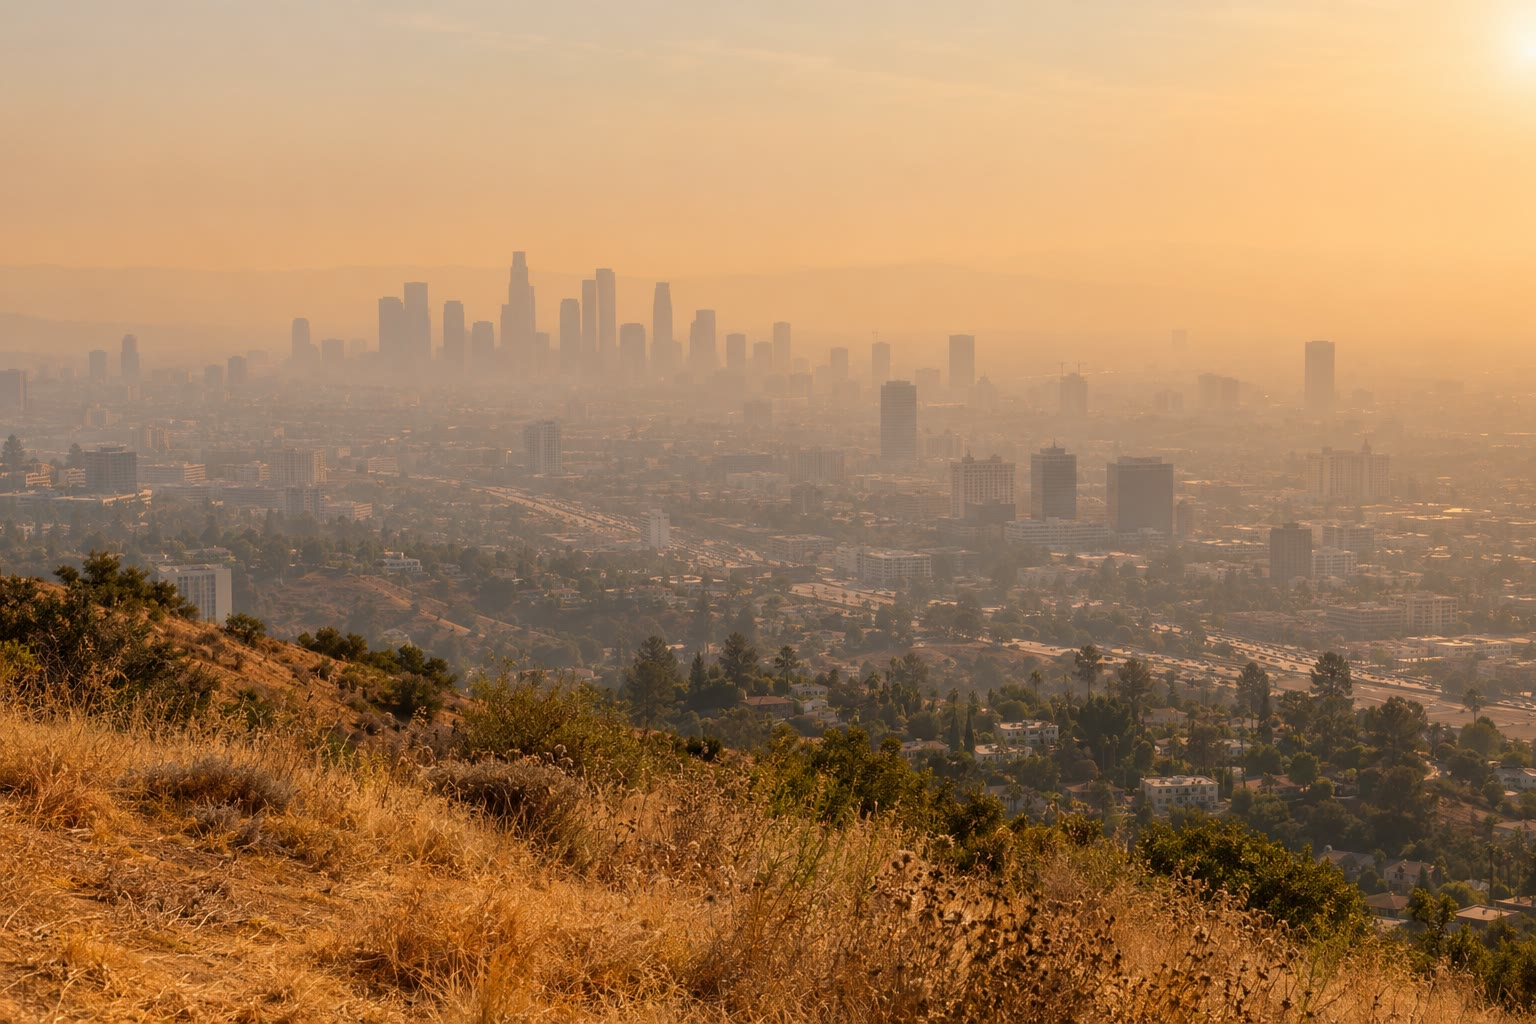
\includegraphics[width=0.6\linewidth]{images/book4/ai/b3-14-smog.jpg}

{\small Uma cidade sob \omterm{def:b3:photochemistry:smog}{smog fotoquímico} em uma tarde quente. A cor castanha vem
do \ce{NO2}; o ozônio, que irrita os pulmões, é invisível.}
\end{omfigure}

\begin{omfigure}
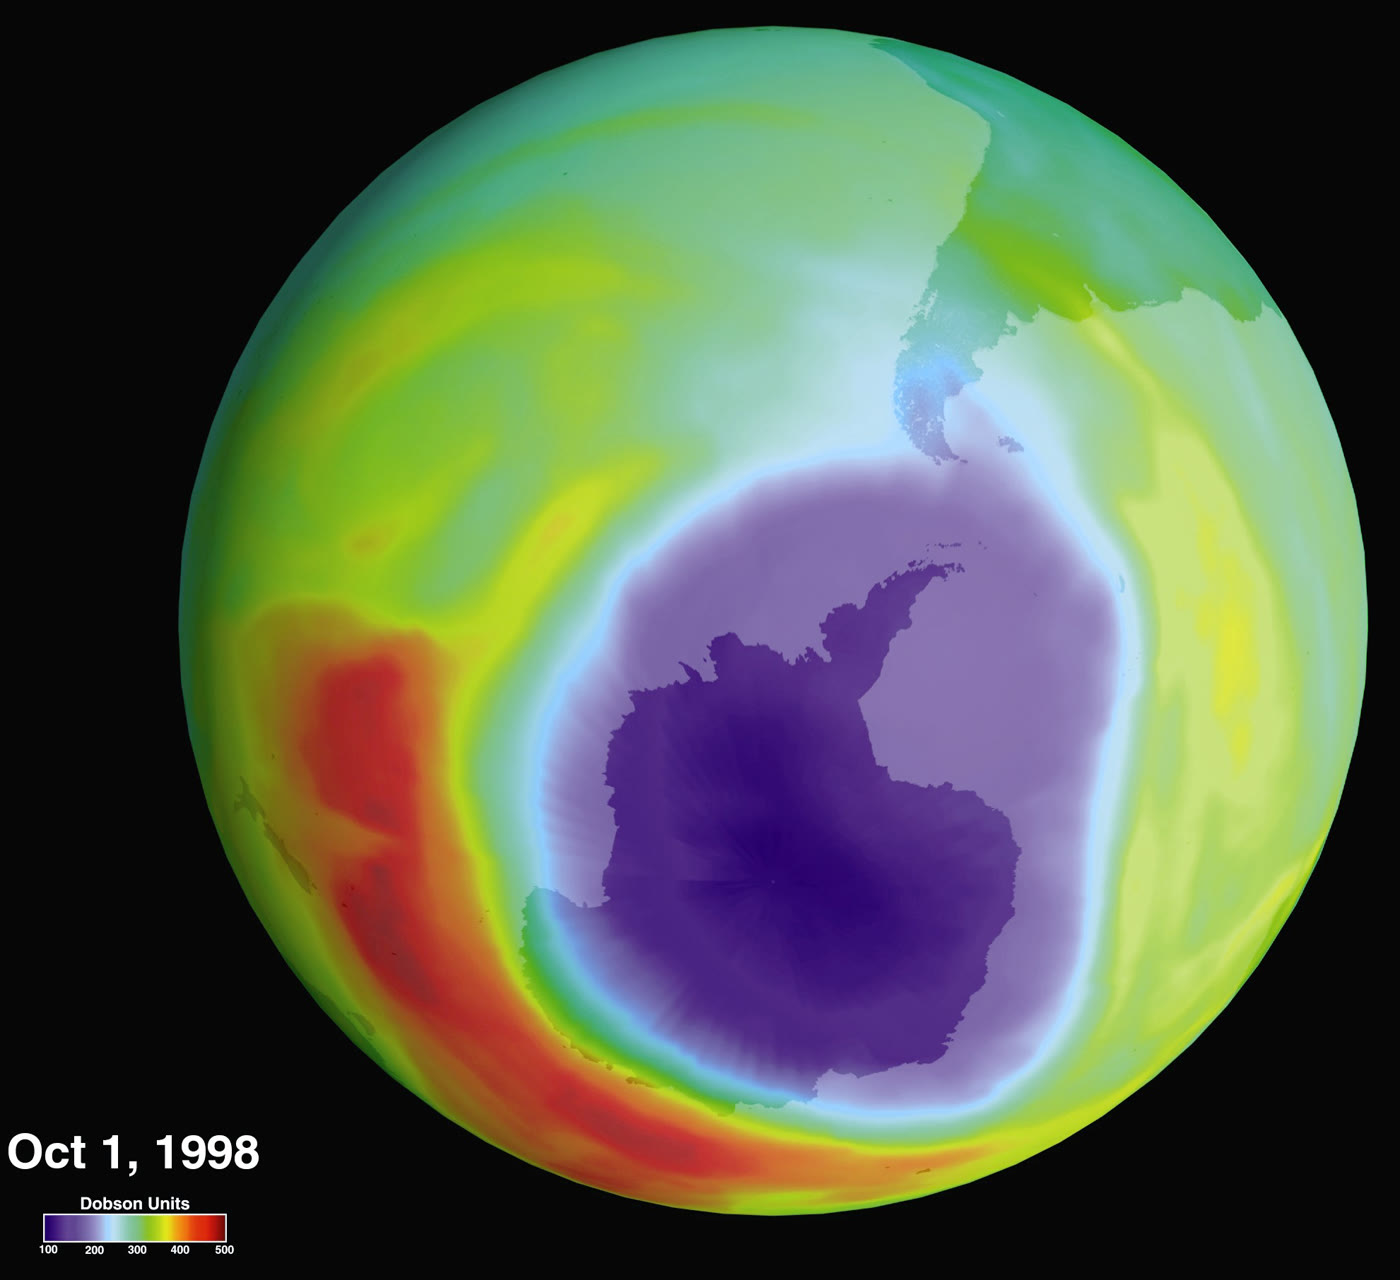
\includegraphics[width=0.5\linewidth]{images/book4/ozone-hole.jpg}

{\small A coluna de ozônio sobre o hemisfério sul em 1.º de outubro de 1998, a partir
de medidas de satélite: o buraco de ozônio sobre a Antártida (roxo) cai para cerca
de 100 unidades Dobson, contra cerca de 300 em outros lugares.}
\end{omfigure}

\begin{inthelab}[Um fotorreator]
Uma lâmpada de mercúrio de média pressão, resfriada em uma camisa de quartzo,
fica no centro do recipiente de reação; uma luva de vidro filtrante remove os
comprimentos de onda abaixo de cerca de \qty{300}{nm}, que destruiriam os produtos.
A solução é desoxigenada com uma corrente de nitrogênio (o oxigênio suprime os
tripletos) e agitada. Todo o reator é enclausurado: a lâmpada emite luz
ultravioleta nociva para os olhos e a pele, e nunca é olhada, nem por um instante.
\end{inthelab}

\begin{safety}{\ghs[0.8cm]{GHS08}\ghs[0.8cm]{GHS09}}
% ledger: ghs4:benzophenone
Benzofenona, um sensibilizador comum e o reagente da fotorredução: suspeita de
provocar câncer, pode afetar órgãos por exposição prolongada, tóxica para os
organismos aquáticos. Pesada e manipulada com luvas; os resíduos vão para o
recipiente de resíduos orgânicos.
\end{safety}

\begin{history}[A fotoquímica do futuro e o buraco no céu]
Em 1912, Giacomo Ciamician, em Bolonha, perguntou se a indústria poderia um dia
funcionar com a luz do Sol, como as plantas, em vez de carvão; ele havia passado
anos expondo ao sol frascos de compostos orgânicos no telhado de seu laboratório.
Em 1985, três cientistas que trabalhavam em uma estação de pesquisa na Antártida
relataram que a coluna de ozônio da primavera acima dela vinha caindo
abruptamente desde o fim dos anos 1970.
O buraco na \omterm{def:b3:photochemistry:chapman}{camada de ozônio}, explicado em poucos anos pela química deste
capítulo, levou à eliminação progressiva dos clorofluorocarbonos.
\end{history}

\section{Exercícios}

\begin{exercise}[$\star$]\label{exo:b3:photochemistry:1}
Uma lâmpada fornece \qty{100}{mW} em \qty{365}{nm}. Quantos fótons por segundo, e
quantos einstein por segundo?
\end{exercise}

\begin{exercise}[$\star$]\label{exo:b3:photochemistry:2}
Em \qty{10.0}{min}, uma solução que absorve \qty{1.00e-7}{einstein.s^{-1}} converte
\qty{2.0e-5}{mol} de reagente. Calcule o \omterm{def:b3:electronic-spectroscopy:quantum-yield}{rendimento quântico}.
\end{exercise}

\begin{exercise}[$\star$]\label{exo:b3:photochemistry:3}
A reação fotoquímica de \ce{H2} com \ce{Cl2} tem \omterm{def:b3:electronic-spectroscopy:quantum-yield}{rendimentos quânticos} de até $10^4$
e mais. O que isso mostra? Escreva as etapas de propagação.
\end{exercise}

\begin{exercise}[$\star$]\label{exo:b3:photochemistry:4}
% ledger: janaf:O.dfH0, janaf:O3.dfH0
A partir das entalpias de formação a 0 K de O (\qty{246.79}{kJ/mol}) e de \ce{O3}
(\qty{145.35}{kJ/mol}), calcule os maiores comprimentos de onda capazes de dissociar
\ce{O2} em dois átomos e \ce{O3} em \ce{O2} e O.
\end{exercise}

\begin{exercise}[$\star\star$]\label{exo:b3:photochemistry:5}
Um fotointerruptor tem, em \qty{365}{nm}, $\varepsilon_E = 22\,000$ e $\varepsilon_Z = 1500$ \unit{L.mol^{-1}.cm^{-1}}, com
$\Phi_{E\to Z} = 0.11$ e $\Phi_{Z\to E} = 0.40$ (dados do exercício). Calcule a composição
fotoestacionária.
\end{exercise}

\begin{exercise}[$\star\star$]\label{exo:b3:photochemistry:6}
Dê os produtos da \omterm{def:b3:photochemistry:norrish}{reação de Norrish do tipo II} da hexan-2-ona e explique por que
a pentan-2-ona dá eteno em vez de propeno.
\end{exercise}

\begin{exercise}[$\star\star$]\label{exo:b3:photochemistry:7}
Um aceptor tem uma energia de tripleto de \qty{250}{kJ/mol}. Entre três
sensibilizadores candidatos com energias de tripleto de 289, 253 e \qty{236}{kJ/mol}
(dados do exercício), qual transfere com eficiência? Estime a constante de
equilíbrio da transferência para cada um a \qty{298}{K}.
\end{exercise}

\begin{exercise}[$\star\star$]\label{exo:b3:photochemistry:8}
% ledger: kin:O+O2+M.k0, kin:O+O2+M.n
A \qty{230}{K}, com $[\mathrm M] = \qty{4.0e17}{cm^{-3}}$, $[\ce{O2}] = 0.21[\mathrm M]$ e $j_3 = \qty{1.0e-3}{s^{-1}}$,
calcule $k_2$ e a razão estacionária $[\ce{O}]/[\ce{O3}]$.
\end{exercise}

\begin{exercise}[$\star\star$]\label{exo:b3:photochemistry:9}
% ledger: kin:Cl+O3.A, kin:Cl+O3.EaR, kin:Cl+CH4.A, kin:Cl+CH4.EaR
A \qty{230}{K}, calcule as constantes de velocidade de $\ce{Cl + O3}$ e de $\ce{Cl + CH4}$, e a
probabilidade de que um átomo de Cl encontre \ce{O3} em vez de \ce{CH4} quando $[\ce{O3}] = \qty{5.7e12}{cm^{-3}}$
e $[\ce{CH4}] = \qty{4.0e11}{cm^{-3}}$.
\end{exercise}

\begin{exercise}[$\star\star\star$]\label{exo:b3:photochemistry:10}
% ledger: kin:NO+O3.A, kin:NO+O3.EaR
Ao meio-dia em uma cidade, $[\ce{NO2}]/[\ce{NO}] = 1.5$ e $j_{\ce{NO2}} = \qty{8.0e-3}{s^{-1}}$. Calcule o
ozônio fotoestacionário a \qty{298}{K} em moléculas por \unit{cm^3} e em ppb (ar a \qty{1}{bar}).
O que acontece à noite?
\end{exercise}

\begin{exercise}[$\star\star\star$]\label{exo:b3:photochemistry:11}
Uma solução de \qty{3.0}{mL} de absorbância 0.50 em \qty{313}{nm} recebe \qty{50}{mW} de
luz nesse comprimento de onda; a reação tem $\Phi = 0.25$. Calcule a velocidade inicial em
\unit{mol.L^{-1}.s^{-1}}.
\end{exercise}

\begin{exercise}[$\star\star\star$]\label{exo:b3:photochemistry:12}
Um actinômetro de ferrioxalato, com \omterm{def:b3:electronic-spectroscopy:quantum-yield}{rendimento quântico} de 1.25 em \qty{365}{nm} (dados
do exercício) e absorção total, forma \qty{3.0e-6}{mol} de Fe(II) em \qty{60}{s}.
Calcule o \omterm{def:b3:photochemistry:photon-flux}{fluxo de fótons}. Por que a conversão deve permanecer pequena?
\end{exercise}

\section{Problema: Fazer e desfazer a camada de ozônio}

\begin{problem}[{Problema de fim de semana --- fazer e desfazer a camada de ozônio:
limiares de fótons, o estado estacionário de Chapman com constantes de velocidade
avaliadas, o ciclo do cloro e os reservatórios que o interrompem}]
\label{pb:b3:photochemistry:1}
% ledger: janaf:O.dfH0, janaf:O3.dfH0, kin:O+O2+M.k0, kin:O+O2+M.n, kin:O+O3.A, kin:O+O3.EaR, kin:Cl+O3.A, kin:Cl+O3.EaR, kin:O+ClO.A, kin:O+ClO.EaR, kin:Cl+CH4.A, kin:Cl+CH4.EaR, kin:ClO+NO2+M.k0, kin:ClO+NO2+M.n, kin:ClO+NO2+M.kinf, kin:ClO+NO2+M.Fc, oz:column.mean, oz:column.hole
Um modelo da estratosfera perto de \qty{30}{km} (dados do problema): $T = \qty{230}{K}$, $[\mathrm M] =
\qty{4.0e17}{cm^{-3}}$, $[\ce{O2}] = 0.21[\mathrm M]$, \omterm{def:b3:photochemistry:photolysis}{constantes de velocidade de fotólise} $j_1 = \qty{1.0e-11}{s^{-1}}$ (\ce{O2})
e $j_3 = \qty{1.0e-3}{s^{-1}}$ (\ce{O3}), $[\ce{CH4}] = \qty{4.0e11}{cm^{-3}}$, $[\ce{NO2}] = \qty{1.0e9}{cm^{-3}}$. Constantes de
velocidade avaliadas (\unit{cm^3.s^{-1}}, ou \unit{cm^6.s^{-1}} para $k_2$, com as concentrações contadas por \unit{cm^3}):
$k_2 = \num{6.0e-34}(T/300)^{-2.6}$; $k_4 = \num{8.0e-12}\eu^{-2060/T}$; Cl + \ce{O3}: $\num{2.8e-11}\eu^{-250/T}$;
O + ClO: $\num{2.5e-11}\eu^{110/T}$; Cl + \ce{CH4}: $\num{6.6e-12}\eu^{-1240/T}$; ClO + \ce{NO2} + M: $\num{1.41e-13}$ nessas
condições.

\medskip\noindent\textbf{Parte I --- Limiares de fótons.}
\begin{enumerate}
  \item Calcule $D_0(\ce{O2})$ a partir de $\Delta_fH^\circ_0(\ce{O}) = \qty{246.79}{kJ/mol}$.
  \item Deduza o maior comprimento de onda capaz de dissociar \ce{O2}.
  \item Calcule a energia de $\ce{O3 -> O2 + O}$ ($\Delta_fH^\circ_0(\ce{O3}) = \qty{145.35}{kJ/mol}$) e seu
        comprimento de onda limiar.
  \item A luz visível poderia, portanto, dissociar o ozônio; por que é a absorção
        ultravioleta do ozônio que importa para a vida?
  \item Por que o \ce{O2} só é fotolisado no alto da atmosfera?
\end{enumerate}

\medskip\noindent\textbf{Parte II --- O estado estacionário de Chapman.}
\begin{enumerate}[resume]
  \item Escreva as quatro etapas de Chapman.
  \item Calcule $k_2$ e $k_2[\mathrm M]$ a \qty{230}{K}.
  \item Calcule $k_4$.
  \item Calcule $[\ce{O}]/[\ce{O3}]$.
  \item Mostre que $[\ce{O3}] = [\ce{O2}]\sqrt{j_1k_2[\mathrm M]/(j_3k_4)}$.
  \item Calcule $[\ce{O3}]$ e sua razão de mistura.
  \item Calcule $[\ce{O}]$.
  \item O ozônio observado é menor que esse valor. Por quê?
\end{enumerate}

\medskip\noindent\textbf{Parte III --- O ciclo do cloro.}
\begin{enumerate}[resume]
  \item Escreva o ciclo e sua reação global.
  \item Calcule o tempo de vida de um átomo de Cl frente ao \ce{O3}.
  \item Calcule o tempo de vida do ClO frente ao O.
  \item Deduza a razão estacionária $[\ce{ClO}]/[\ce{Cl}]$.
  \item Com $[\ce{Cl}] + [\ce{ClO}] = \qty{1.0e7}{cm^{-3}}$, compare a velocidade de perda de oxigênio
        ímpar pelo ciclo com a da etapa de Chapman $\ce{O + O3}$.
  \item Que etapa limita o ciclo?
\end{enumerate}

\medskip\noindent\textbf{Parte IV --- Os reservatórios.}
\begin{enumerate}[resume]
  \item Calcule a probabilidade de que um átomo de Cl reaja com \ce{O3} em vez de com
        \ce{CH4}.
  \item Calcule a probabilidade de que o ClO reaja com O em vez de com \ce{NO2}.
  \item Deduza a probabilidade $p$ de que uma volta do ciclo se complete.
  \item Deduza o número médio de voltas antes que o cloro seja capturado.
  \item Explique como as nuvens estratosféricas polares alongam a cadeia.
  \item Enuncie o resultado: o número de moléculas de ozônio que um átomo de cloro
        destrói, nesse modelo, antes de ser capturado em um reservatório.
\end{enumerate}
\end{problem}
